% ============ 5 景 (原书 pp.38-41) ============
\chapter{景}\label{sec:5}

% 脚注中的交换图用显式坐标的 tikzpicture (不用 tikzcd: 其矩阵 & 无法出现在宏参数/脚注中)
\newcommand{\FbCXdiagram}{%
  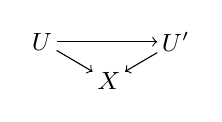
\begin{tikzpicture}[baseline=(current bounding box.center), every node/.style={inner sep=1.5pt, font=\small}]
    \node (U) at (0, 0.5) {$U$};
    \node (Up) at (1.7, 0.5) {$U'$};
    \node (X) at (0.85, 0) {$X$};
    \draw[->] (U) -- (Up);
    \draw[->] (U) -- (X);
    \draw[->] (Up) -- (X);
  \end{tikzpicture}}
\newcommand{\FbFibdiagram}{%
  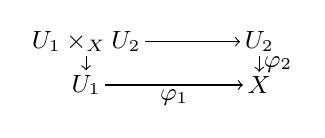
\begin{tikzpicture}[baseline=(current bounding box.center), every node/.style={inner sep=1.5pt, font=\small}]
    \node (A) at (0, 0.55) {$U_1 \times_{X} U_2$};
    \node (U2) at (2.2, 0.55) {$U_2$};
    \node (U1) at (0, 0) {$U_1$};
    \node (X) at (2.2, 0) {$X$};
    \draw[->] (A) -- (U2);
    \draw[->] (A) -- (U1);
    \draw[->] (U2) -- (X) node[midway, right, font=\small] {$\varphi_2$};
    \draw[->] (U1) -- (X) node[midway, below, font=\small] {$\varphi_1$};
  \end{tikzpicture}}
\index{景}
\index{Grothendieck 拓扑}
\index{预层}
\index{层}
\index{平展景}
\index{平坦景}
\index{有限平展拓扑}
\index{完全分解拓扑}
\index{筛}
\index{意象}
\index{连续映射}

为了发展层论以及层的上同调理论(例如在 Grothendieck 1957 年 T\^ohoku 论文中那样)，并不需要有通常意义下的拓扑空间.事实上，只需有一个范畴 $C$ 连同：对 $C$ 的每个对象 $U$，一族特异映射族 $(U_i \to U)_{i \in I}$，称为 $U$ 的覆盖，满足下列公理：
\begin{enumerate}
  \item 对任何覆盖 $(U_i \to U)_{i \in I}$ 和 $C$ 中的任何态射 $V \to U$，纤维积\footnote{对范畴 $C$ 的对象 $X$，$C/X$ 表示对象为 $C$ 中态射 $U \to X$，箭头为交换图
  \begin{center}
  \FbCXdiagram
  \end{center}
  的范畴.使此图交换的态射 $U \to U'$ 也称为 $X$-态射.$C$ 中态射 $\varphi_1 \colon U_1 \to X$，$\varphi_2 \colon U_2 \to X$ 的纤维积 $U_1 \times_{X} U_2$ 是它们在范畴 $C/X$ 中的积.于是，有交换图
  \begin{center}
  \FbFibdiagram
  \end{center}
  具有明显的泛性质.}$U_i \times_{U} V$ 存在，且 $(U_i \times_{U} V \to V)_{i \in I}$ 是 $V$ 的覆盖；
  \item 若 $(U_i \to U)_{i \in I}$ 是 $U$ 的覆盖，且对每个 $i \in I$，$(V_{ij} \to U_i)_{j \in J_i}$ 是 $U_i$ 的覆盖，则族 $(V_{ij} \to U)_{i, j}$ 是 $U$ 的覆盖；
  \item 对 $C$ 中任何 $U$，由单个映射组成的族 $\left(U \xrightarrow{\mathrm{id}} U\right)$ 是 $U$ 的覆盖.
\end{enumerate}
在 (b) 中，映射 $V_{ij} \to U$ 是 $V_{ij} \to U_i \to U$ 的复合.

覆盖系统这时称为 (Grothendieck) 拓扑，而 $C$ 连同该拓扑称为景.若 $T$ 是景，则 $\mathrm{Cat}(T)$ 表示其底层范畴.

例如，设 $X$ 是拓扑空间，$C$ 是对象为 $X$ 的开子集，态射为包含映射的范畴.则族 $(U_i \to U)_{i \in I}$ 且 $(U_i)_{i \in I}$ 是 $U$ 的开覆盖，构成 $C$ 上的 Grothendieck 拓扑.对 $V$ 的开子集 $U$ 与 $U'$，$U \times_{V} U' = U \cap U'$.

景 $T$ 上的集合预层是反变函子 $F \colon \mathrm{Cat}(T) \to \mathbf{Sets}$.于是，对 $\mathrm{Cat}(T)$ 中每个对象 $U$，$F$ 配给一个集合 $F(U)$，对 $\mathrm{Cat}(T)$ 中每个态射 $\varphi \colon U \to V$，配给映射 $F(\varphi) \colon F(V) \to F(U)$，使得 $F(\psi \circ \varphi) = F(\varphi) \circ F(\psi)$ 且 $F(\mathrm{id}_{U}) = \mathrm{id}_{F(U)}$.注意 $T$ 上预层的概念不依赖于覆盖.我们有时把 $F(\varphi) \colon F(V) \to F(U)$ 写为 $a \mapsto a|_{U}$，尽管这可能引起混淆，因为可能有多于一个态射 $U \to V$.

类似地，$T$ 上的(阿贝尔)群或环预层是从 $\mathrm{Cat}(T)$ 到(阿贝尔)群或环范畴的反变函子.

$T$ 上的层是满足层条件的预层 $F$：
\[
(\mathrm{S}) \colon \quad F(U) \to \prod_{i \in I} F(U_i) \rightrightarrows \prod_{(i, j) \in I \times I} F(U_i \times_{U} U_j)
\]
对每个覆盖 $(U_i \to U)$ 正合.于是，$F$ 是层，如果映射
\[
f \mapsto (f|_{U_i}) \colon F(U) \to \prod F(U_i)
\]
把 $F(U)$ 等同于乘积中由这样的族 $(f_i)$ 组成的子集：对所有 $i, j \in I \times I$，
\[
f_i|_{U_i \times_{U} U_j} = f_j|_{U_i \times_{U} U_j}.
\]

当 $T$ 是由拓扑空间产生的景时，这些定义与通常的定义一致.

预层的态射就是函子的态射(又名自然变换)，层的态射是预层的态射.

现在我们列出一些景.本节余下部分中，$X$ 是簇或概形.簇的正则映射族 $(\varphi_i \colon U_i \to U)$ 称为满的，如果 $U = \bigcup \varphi_i(U_i)$，概形的态射族类似.

\textbf{$X$ 上的 Zariski 景} 景 $X_{\mathrm{zar}}$ 是与把 $X$ 看作 Zariski 拓扑的拓扑空间相联系(如上)的景.

\textbf{$X$ 上的平展景} 景 $X_{\mathrm{et}}$ 的底层范畴是 $\mathbf{Et}/X$，其对象是平展态射 $U \to X$，箭头是 $X$-态射 $\varphi \colon U \to V$.覆盖是 $\mathbf{Et}/X$ 中平展态射的满族 $(U_i \to U)$.

\textbf{$X$ 上平展景的变体} 显然，在 Grothendieck 的原始定义中，覆盖取为映射族 $(U_i \to U)_{i \in I}$ 的满族，其中每个映射都是到 $U$ 的某个 Zariski 开子集上的有限平展映射.换言之，定义选取的方式使对该拓扑为``平凡''与 Serre 术语中的``等平凡''一致(见引言).这就是有限平展拓扑，相应的景记为 $X_{\mathrm{fet}}$.\footnote{正确的定义是由 Artin 向他建议的.}

另一个变体由 Nisnevich 提出，它在 $K$ 理论和群概形上同调的研究中被证明有用.它取平展映射的满族 $(U_i \to U)_{i \in I}$ 为覆盖，这些映射有如下性质：对每个 $u \in U$，存在 $i \in I$ 与 $u_i \in U_i$，使得剩余域上的映射 $\kappa(u) \to \kappa(u_i)$ 是同构.该条件对所有 $u \in U$(包括非闭点)都施加，因此即使对代数闭域上的簇，这也不同于平展拓扑.它称为完全分解拓扑，相应的景记为 $X_{\mathrm{cd}}$.$X$ 的点 $x$ 处该拓扑的局部环是 $\mathcal{O}_{X, x}$ 的 Hensel 化(而不是严格 Hensel 化).

在下面两个例子中，我们取 $X$ 为概形.

\textbf{$X$ 上的平坦景} 景 $X_{\mathrm{Fl}}$ 的底层范畴是 $\mathbf{Sch}/X$，即所有 $X$-概形的范畴.覆盖是 $X$-态射的满族 $\left(U_i \xrightarrow{\varphi_i} U\right)$，其中每个 $\varphi_i$ 平坦且有限型.

\textbf{$X$ 上的大平展景} 景 $X_{\mathbf{Et}}$ 的底层范畴是 $\mathbf{Sch}/X$.覆盖是平展 $X$-态射的满族 $(U_i \to U)_{i \in I}$.

\textbf{景 $T_G$} 对每个 pro-有限群 $G$，对应一个景 $T_G$，其底层范畴是 $G$ 的一切有限离散集合的范畴.覆盖是 $G$-映射的任何满族.

\begin{remark}\label{rem:5.1}
(a) 当 $U \to X$ 是 $X$ 的某个覆盖的成员时，我们可以把 $U$ 看作该``拓扑''的 $X$ 的``开子集''.然而注意，对平坦景，$U \to X$ 与 $U' \to X$ 可能都是 $X$ 的``开子集''，但 $X$-态射 $U \to U'$ 可能不把 $U$ 实现为 $U'$ 的``开子集''，即 $U \to X$ 与 $U' \to X$ 可以平坦而 $U \to U'$ 不平坦.

(b) 若底层范畴中的所有概形都拟紧(例如簇)，则可以把覆盖取为有限满族.
\end{remark}

\begin{definition}\label{def:5.2}
设 $T_1$ 与 $T_2$ 是两个景.保持纤维积并把覆盖变为覆盖的函子 $\mathrm{Cat}(T_2) \to \mathrm{Cat}(T_1)$ 称为连续映射 $T_1 \to T_2$.
\end{definition}

例如，拓扑空间的映射 $Y \to X$ 定义相应景的连续映射，当且仅当它按通常意义连续.

有显然的景的连续映射
\[
X_{\mathrm{Fl}} \to X_{\mathbf{Et}} \to X_{\mathrm{et}} \to X_{\mathrm{cd}} \to X_{\mathrm{zar}}.
\]
若 $X = \operatorname{Spec} k$($k$ 是域)，且 $k^{\mathrm{sep}}$ 是 $k$ 的代数闭包，则存在本质互逆的连续映射
\[
T_G \to X_{\mathrm{et}}, \qquad X_{\mathrm{et}} \to T_G,
\]
其中 $G = \operatorname{Gal}(k^{\mathrm{al}}/k)$---见 \S 3.

\begin{remark}\label{rem:5.3}
注意，连续映射 $T_1 \to T_2$ 实际上是反方向的函子.这在 SGA 4 的参与者看来太不合逻辑了，于是他们把连续映射 $T_1 \to T_2$ 定义为保持覆盖的函子 $\mathrm{Cat}(T_1) \to \mathrm{Cat}(T_2)$.然而，这与我们从拓扑空间获得的直觉冲突，在出版版本中被放弃了.
\end{remark}

\textbf{术语对照} 我们称为拓扑的东西在 SGA 4 中称为预拓扑.在那里他们把筛(法语 crible)定义为全子范畴\footnote{这意味着子范畴中的 Hom 集等于所在范畴中的 Hom 集.}，它随任何对象 $V$ 一起包含所有允许到 $V$ 的态射的对象.在 SGA 4 的意义下给范畴 $C$ 一个拓扑，就是给 $C$ 的每个对象 $U$ 一组满足某些自然公理的 $C/U$ 中的筛(同上，II.1).在 SGA 4 中，景被定义为带这种意义的拓扑的范畴.

设 $T$ 是按本节开头定义的景.对任何覆盖 $\mathcal{U} = (U_i \to U)_{i \in I}$，配上筛 $\mathfrak{s}(\mathcal{U})$，其对象是 $\mathrm{Cat}(T)$ 中允许到某个 $U_i$ 的态射的那些对象.由覆盖产生的筛定义了 SGA 4 意义下的拓扑.

意象是等价于景上层范畴的任何范畴.在 SGA 4, p.299 中，论证了意象比景更适合作为研究对象.然而，我在本讲义中不再使用这个词.

有理由更喜欢预拓扑而非拓扑和意象.例如，所有概形范畴上的平展与光滑预拓扑定义相同的层范畴，但给出不同的``局部''概念.见 de Jong 2010 年 6 月 18 日的博客文章.在 Stacks Project 中，他们把景定义为带预拓扑的范畴.
